\documentclass[12pt]{article}
\usepackage{epsf,epic,eepic,eepicemu}
%\documentstyle[epsf,epic,eepic,eepicemu]{article}
\usepackage[utf8]{inputenc}

\usepackage{graphicx}

\begin{document}
%\oddsidemargin=-5mm \evensidemargin=-5mm \marginparwidth=.08in
%\marginparsep=.01in \marginparpush=5pt \topmargin=-15mm
%\headheight=12pt \headsep=25pt \footheight=12pt \footskip=30pt
%\textheight=25cm \textwidth=17cm \columnsep=2mm \columnseprule=1pt
%\parindent=15pt\parskip=2pt

\begin{center}
\bf Semestrální projekt MI-PPR.2 2014/2015\\[5mm]
    Paralelní algoritmus pro řešení problému Permutace číselných kostek\\[5mm]
       Vojtěch Drbohlav\\[2mm]
magisterské studium, FIT ČVUT, Kolejní 550/2, 160 00 Praha 6\\[2mm]
\today
\end{center}

\section{Definice problému}

\subsection{Vstupní data}

a,b = přirozená čísla, a\textgreater=b\textgreater=3\\
q = přirozené číslo, a*b{\textgreater}q\\
X0 = počáteční konfigurace zkonstruovaná zpětným provedením q náhodných tahů z cílové konfigurace. Platí q\textgreater=d(X0). 

\begin{center}
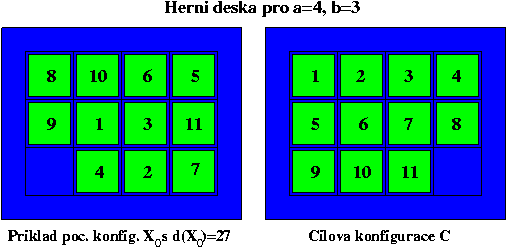
\includegraphics[width=10cm]{pec}
\end{center}

\subsection{Definice}

Je-li X konfigurace, daná rozmístěním číselných kostek na herní desce, pak
t(X) je počet doposud provedených tahů, kterými jsme převedli počáteční konfiguraci X0 na konfiguraci X.
d(X) je spodní mez počtu tahů, kterými se lze dostat z konfigurace X do cílové konfigurace C. Tato spodní mez je rovna manhatanské vzdálenosti X od cílové konfigurace C, což je součet manhatanských vzdáleností současného a cílového políčka všech kostek. Manhatanská vzdálenost políček (x1,y1) a (x2,y2) je {\textbar}x1-x2{\textbar}+{\textbar}y1-y2{\textbar}. Spodní mez počtu tahů nejlepšího možného řešení je tedy d(X0).

\subsection{Pravidla a cíl hry}

Pravoúhlá herní deska se skládá z a x b čtvercových políček, v kterých jsou na počátku podle určité permutace rozmístěny po řádcích kostky s čísly 1 až M-1, kde M=ab, a jedno políčko se nechá prázdné, viz obrázek vlevo. Tomuto rozmístění kostek budeme říkat počáteční konfigurace X0. Jeden tah je vodorovný nebo svislý posun jedné kostky na sousední volné políčko. Cílem hry je použitím minimálního počtu tahů převést počáteční konfiguraci X0 na cílovou konfiguraci C, ve které jsou kostky seřazeny vzestupně po řádcích a prázdné políčko je vpravo dole, jak ukazuje obrázek vpravo.

\section{Popis sekvenčního algoritmu}

Jedná se o algoritmus typu BB-DFS, tedy prohledávání stavového prostoru do hloubky. Stavový prostor je nekonečný, proto je hloubka zásobníku shora omezena počtem náhodných tahů,k terý byly použity k vygenerování počáteční konfigurace $X_0$. Zezdola je hloubka zásobníku omezena manhatanskou vzdáleností $X$ a $X_0$, tedy $d(X_0)$.

Po inicializaci algoritmu je na vrcholu zásobníku uzel s číslem 0. Nad zásobníkem se poté provádí prohledávání prostoru. Jeden krok algoritmu vypadá takto:

\begin{enumerate}
\item Přečte vrchol zásobníku a zjistí zda se jedná o uzavřený nebo otevřený tah
\item Pokud se jedná o otevřený tah, provede ho, změní jeho typ na uzavřený
\item Zjistí, zda je hra v cílové konfiguraci
\item Pokud ano, tak uloží nové nejlepší řešení a ukončí krok
\item Pokud ne a ještě se nedosáhlo horní meze hloubky zásobníku q a hloubka zásobníku je nižší než délka aktuálně nalezeného nejlepšího řešení, tak přidá na vrchol zásobníku všechny možné tahy, kterými je možné pokračovat ve hře
\item Pokud se jedná o uzavřený tah, tak provede tah v opačném směru a odebere ho z vrcholu zásobníku
\end{enumerate}

Algoritmus končí prázdným zásobníkem.

Vstup program může načíst ze souboru, jeho cestu přečte z prvního spouštěcího argumentu. Také je možné nechat vygenerovat náhodnou počáteční konfiguraci, argumenty programu jsou potom zadány v tomto pořadí: počet řádků stavového prostoru, počet sloupců stavového prostoru a počet náhodných tahů, které se mají provést.

Výstupem programu je počet a posloupnost tahů, které vedou z počáteční konfigurace do cílové konfigurace, a doba výpočtu.

\begin{table}[ht]
\begin{center}
\begin{tabular}{c|c}
  Vstup & Čas \\
  \hline
  input.10m & 648.324 s \\
  input.15m & 885.035 s \\
  input.20m & 1217.23 s \\
\end{tabular}
\end{center}
\caption{Naměřené časy}
\end{table}

\section{Popis paralelního algoritmu a jeho implementace v MPI}

Paralelní algoritmus je v podstatě stejný jako sekvenční, akorát jsem do něj doplnil komunikaci přes MPI, dělení zásobníku a distribuované ukončení výpočtu.

Po spuštění hlavní proces vygeneruje nebo načte počáteční konfiguraci a rozešle ji ostatním procesům, které na ni čekají, po přijetí této konfigurace začnou procesy čekat na část zásobníku. Hlavní proces vygeneruje alespoň tolik oteřených tahů, kolik je procesů, tyto tahy rozešle ostatním procesům a ve svém zásobníku je označí jako odeslané, aby je během výpočtu přeskočil.

Po každých sto krocích prohledávání procesy zpracují zprávy, které jim mohly být zaslány ostatními procesy. Pokud proces najde nové nejlepší řešení rozešle ho ostatním procesům, ty si toto řešení uloží a podle toho mohou více omezit hloubku zásobníku.

Po vyprázdnění zásobníku pošle proces žádost o práci jinému procesu a poté pouze obluhuje příchozí komunikaci. Pokud dostane odpověď, že žádaný proces práci nemá, tak inkrementuje číslo procesu, který žádá o práci modulo počet procesů a pošle žádost znovu. Takto žádá proces o práci dokud nedojde k ukončení výpočtu. Žádaný proces vždy pošle svůj nevyšší otevřený tah procesu, který žádá o práci, a označí tento tah jako odeslaný.

Ukončení výpočtu probíhá cyklickým posíláním peška mezi procesy tak, jak je popsané na eduxu.

\begin{table}[ht]
\begin{center}
\begin{tabular}{c|c|c|c|c}
  Vstup a počet procesů & 2 & 12 & 24 & 32 \\
  \hline
  input.10m & 345.259 s & 60.7551 s & 20.3565 s & 12.0362 s \\
  input.15m & 365.023 s & 87.8443 s & 35.547 s & 6.73745 s \\
  input.20m & 686.029 s & 48.7106 s & 23.5523 s & 10.1069 s \\
\end{tabular}
\end{center}
\caption{Naměřené časy na síti InfiniBand}
\end{table}

\begin{table}[ht]
\begin{center}
\begin{tabular}{c|c|c|c|c}
  Vstup a počet procesů & 2 & 12 & 24 & 32 \\
  \hline
  input.10m & 386.827 s & 58.7045 s & 17.0789 s & 26.6413 s \\
  input.15m & 432.199 s & 86.2835 s & 30.8757 s & 21.7081 s \\
  input.20m & 792.638 s & 49.0979 s & 37.2156 s & 8.18601 s \\
\end{tabular}
\end{center}
\caption{Naměřené časy na síti Ethernet}
\end{table}


\section{Naměřené výsledky a vyhodnocení}

Naměřené časy jsem již uvedl v tabulkách 1, 2 a 3. Při paralelním výpočtu došlo k superlinérnímu zrychlení. Důvodem je to, že při prohledávání stavového prostoru více procesory dojde k nalezení řešení mnohem dříve a úloha se tedy dříve omezí posledním nalezeným nejlepším řešením.

Grafy zrychlení jsou vidět na obrázcích 1 až 6.

\begin{figure}[ht]
\begin{center}
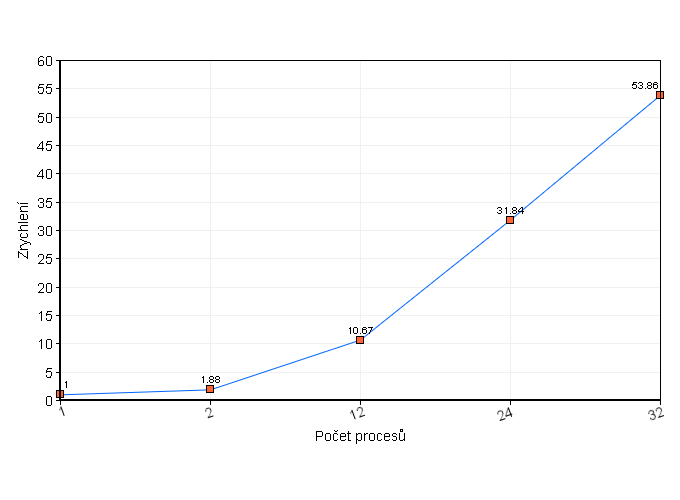
\includegraphics[width=15cm]{input_10m_infiniband}
\end{center}
\caption{Zrychlení pro vstup input.10m na síti InfiniBand}
\end{figure}

\begin{figure}[ht]
\begin{center}
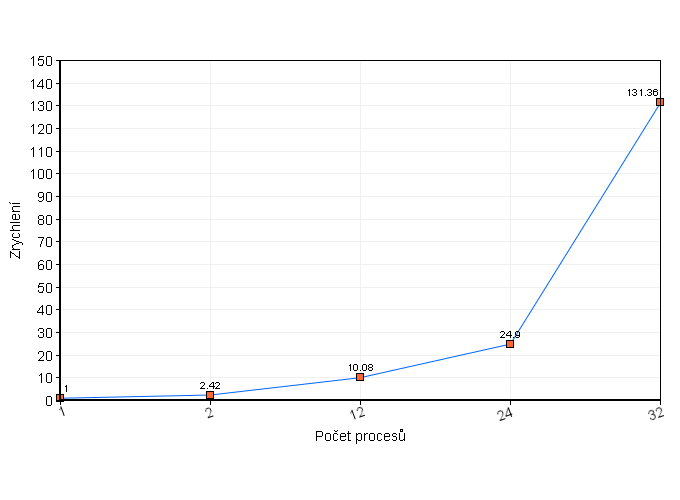
\includegraphics[width=15cm]{input_15m_infiniband}
\end{center}
\caption{Zrychlení pro vstup input.15m na síti InfiniBand}
\end{figure}

\begin{figure}[ht]
\begin{center}
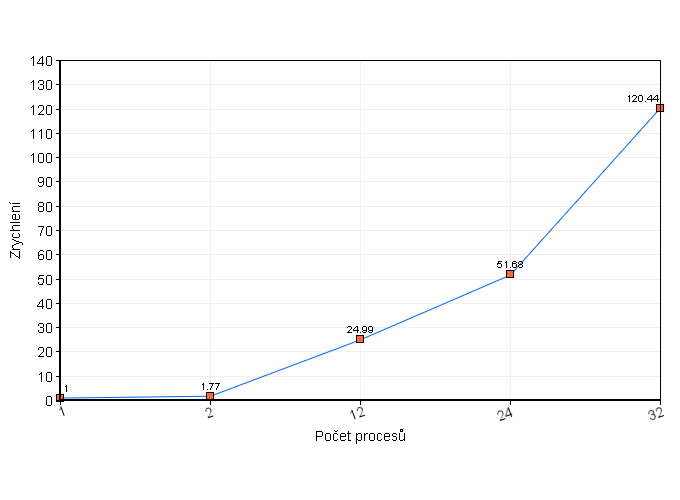
\includegraphics[width=15cm]{input_20m_infiniband}
\end{center}
\caption{Zrychlení pro vstup input.20m na síti InfiniBand}
\end{figure}

\begin{figure}[ht]
\begin{center}
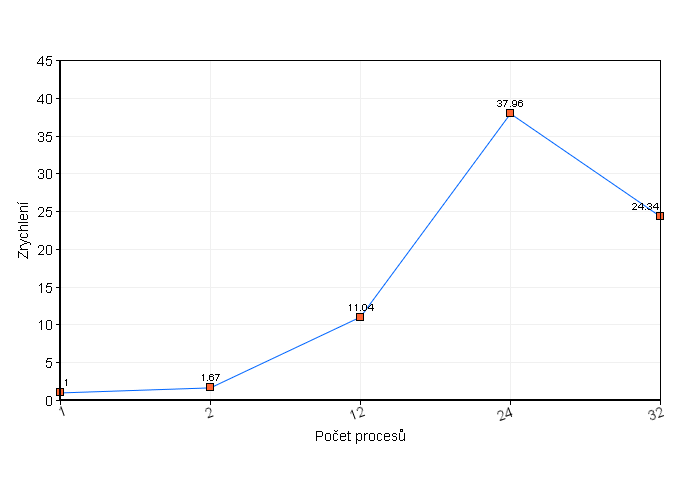
\includegraphics[width=15cm]{input_10m_ethernet}
\end{center}
\caption{Zrychlení pro vstup input.10m na síti Ethernet}
\end{figure}

\begin{figure}[ht]
\begin{center}
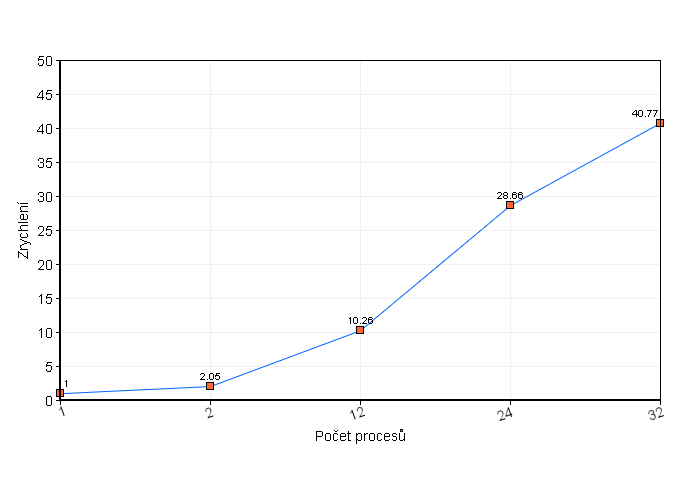
\includegraphics[width=15cm]{input_15m_ethernet}
\end{center}
\caption{Zrychlení pro vstup input.15m na síti Ethernet}
\end{figure}

\begin{figure}[ht]
\begin{center}
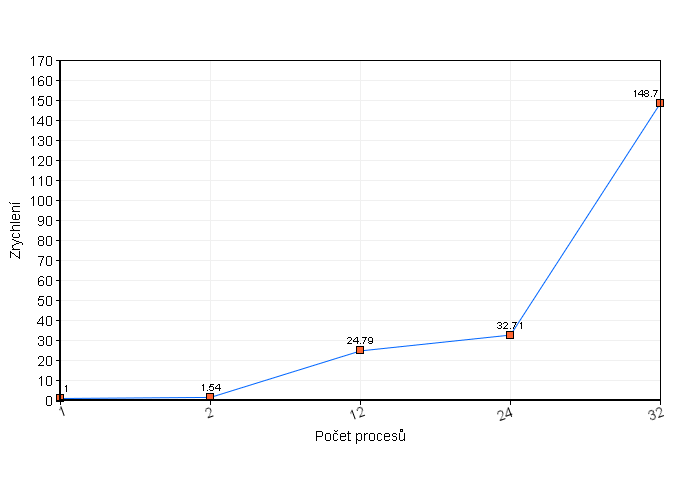
\includegraphics[width=15cm]{input_20m_ethernet}
\end{center}
\caption{Zrychlení pro vstup input.20m na síti Ethernet}
\end{figure}

\begin{enumerate}


\item Z naměřených dat sestavte grafy zrychlení $S(n,p)$. Zjistěte, zda a za jakych podmínek
došlo k superlineárnímu zrychlení a pokuste se je zdůvodnit.

\end{enumerate}

\section{Závěr}

Na semestrální práci by se daly ještě některé věci vylepšit. Mezi ně patří hlavně způsob dělení zásobníku, ten je nyní velmi primitivní, ale z časových důvodů jsem bohužel nestihl naimplementovat žádný chytřejší.

\end{document}